\chapter{Introduction to Distributed systems}

\section{What is a distributed system?}
There is a running joke among the distributed system designers is that the definition of such system is "I can \textbf{NOT} get my work done because some computer somewhere has failed that I never knew existed". More formally a distributed system is such a system that is

\begin{itemize}
    \item running on more than one \textbf{Node}
    \item nodes are interconnected by Computer Networks
    \item characterized by partial failures
\end{itemize}

\noindent Here a \textbf{Node} is a computer or an instance of an application that is running on a computer and \textit{partial failure} means some part of the system is working and some part may not be working.

\section{Failures, problems in distributed systems}

\noindent So a distributed system is defined based on the failure of it's components. So there are many types of failure that should be accounted for. Mainly two broad \textit{philosophy} are used to deal with failures in a distributed system.

\begin{itemize}
    \item \textbf{High-Performance Computing} philosophy where we treat partial failures as total failure and start the entire operation from start or from previously saved checkpoints
    \item \textbf{Cloud Computing} philosophy where we treat the partial failures as a component failure and try to mitigate the fallout from the failure by working around it. The main philosophy here is that every thing fails eventually, so make a system that is \textbf{fault tolerant}.
\end{itemize}

\noindent Consider a two \textbf{Node} system $M_X$ and $M_Y$ is connected via a computer network some distance [1600 KM let's say] apart. Now the machine $M_Y$ has some critical data that $M_X$ needs to get hold of and increment by 1. Think of the failures that can occur during this whole operation.

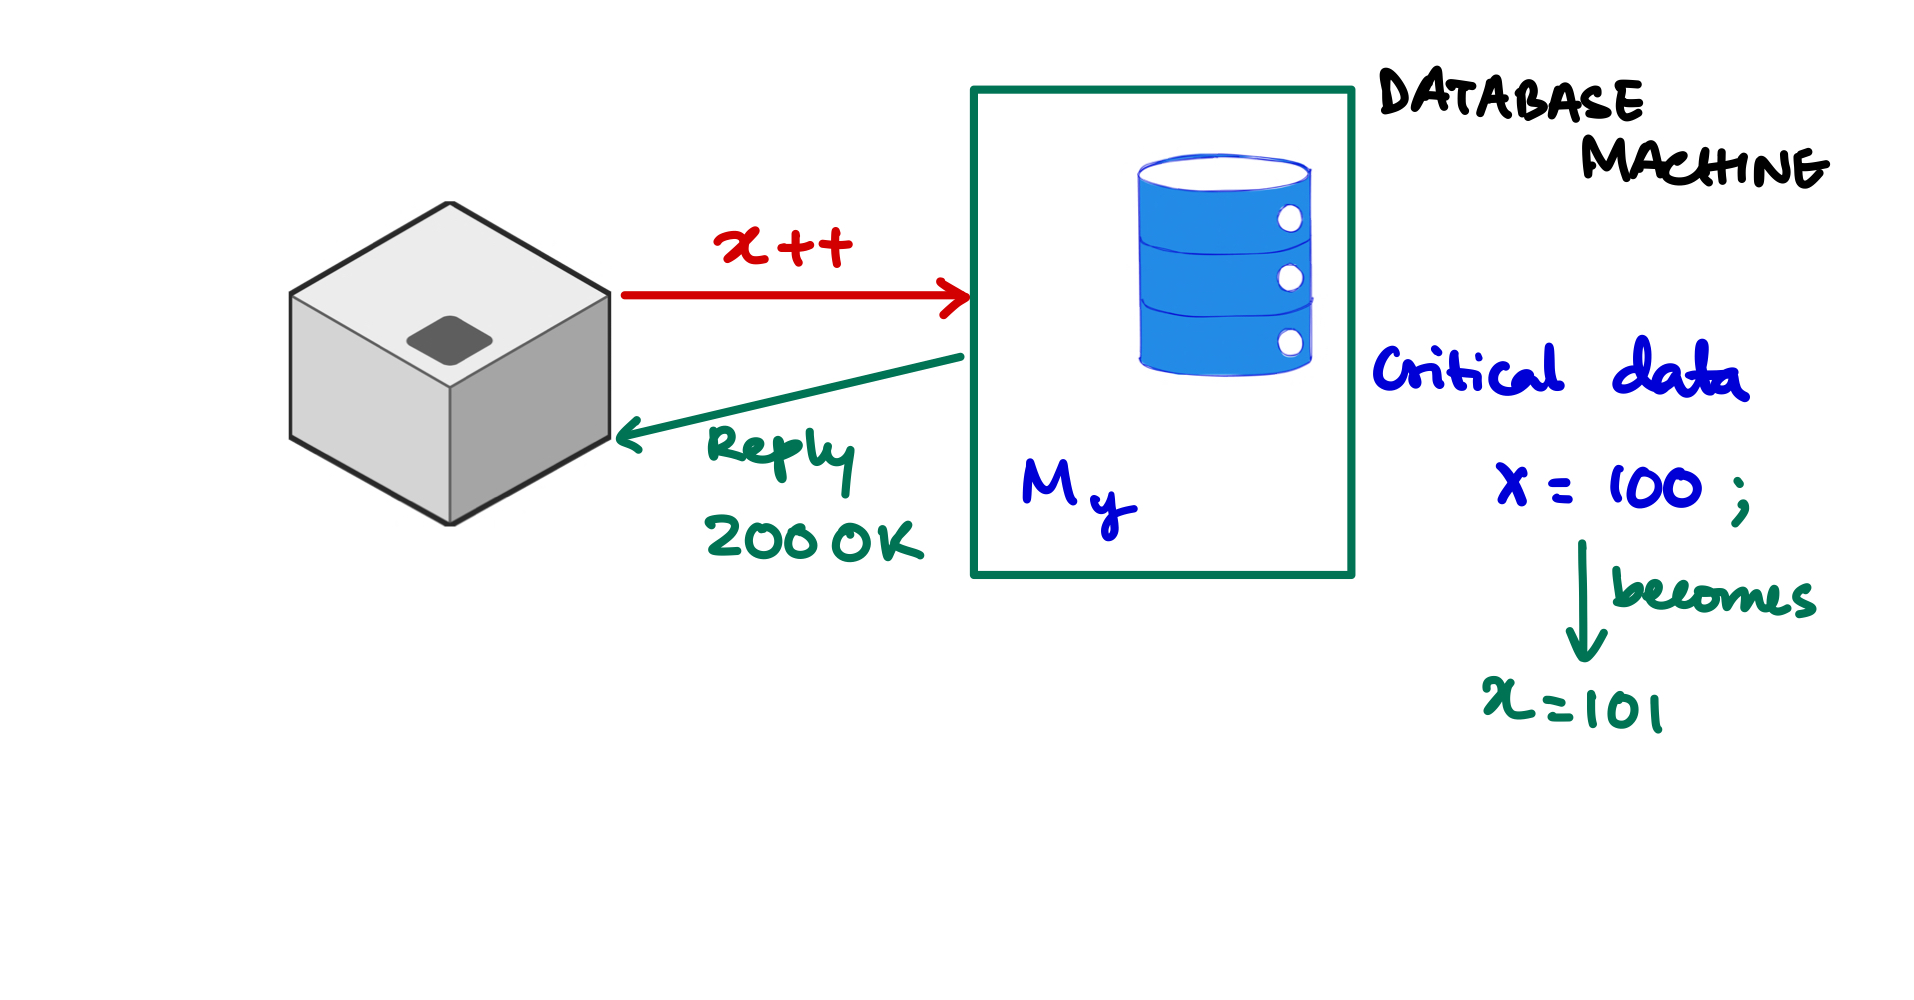
\includegraphics[scale=0.15]{images/img1.jpeg}

\noindent \textbf{Things} that can \textit{fail} in this system are the following
\begin{itemize}
    \item The command \texttt{x++} never transmits to the Machine $M_Y$, gets lost during transit,
    \item $M_Y$ \textit{crashes} during the execution of \texttt{x++} so the reply \texttt{200 OK} never comes back to machine $M_X$,
    \item The command \texttt{x++} gets corrupted in transit,
    \item \texttt{x++} executes alright but the reply \texttt{200 OK} never comes back to machine $M_X$,
    \item \texttt{x++} executes alright but the reply \texttt{200 OK} get corrupted in transit to machine $M_X$,
    \item Value of X got changed while the reply \texttt{200 OK} is in transit back to machine $M_X$
    \item Both the system is running with lot less CPU power than expected rendering the whole system slow.
\end{itemize}

\noindent Although we have so much problems with distributed systems we still make systems distributed for the following reasons \textsc{Reliability of data, high throughput, faster executions}. And \textbf{Yes} if you are thinking that some of those above problems can be solved with TCP in the transport layer of the network, you are absolutely correct.


\section{When to use distributed systems?}
With so many problems in a distributed systems why would anybody having a sane mind would go for a distributed systems though? The answer is pretty simple, you wouldn't unless you \textbf{have to}. When the problem is too big, too heavy to solve even for one machine you will have to solve it with distributed systems. For example let's take the following system:

\noindent Your business is an online exam preparation course (for example say JEE or GATE coaching), you have about 100,000 candidates registered with your course and they study notes from your website, take tests and see their evaluation. Let's see how much load this website gets.
\begin{itemize}
    \item During normal times about 5-8 months before the actual exam website gets about $\approx$ 4000-5000 people in certain hour concurrently watching videos, studying notes and watching solutions, and maybe 500 people are taking short exams on the website's exam portal to prepare.
    \item During an All India Mock test $\approx$ 75000 - 80000 candidates signs on to the portal to give exam and order of 100s of candidate skips the exam to watch videos.
\end{itemize}

\noindent Now if you see, a decent \textbf{AWS} virtual machine server running linux with 8 GB RAM with 4 core CPU and about 200 GB worth of disk space for persistent database would be fine to run during normal times as discussed above. During all india exams we may have to scale the server to 32 GB RAM, and 16 Core CPU to handle all of the candidates. But more or less with one virtual machine it is sufficient for this company to run a multi-crore rupees business online. So they most definitely do not need a distributed system for their business, going distributed is not worth the money and effort to maintain for this case.

\noindent If your business 
\begin{itemize}
    \item handles in the order of 100-200 million requests every minutes,
    \item has 50s, 100s of terabytes of worth of business critical data that must not be lost,
    \item has millions of requests for data delivery half-way accross the world,
    \item too big of a service to fail even for a minute in any given time, date, place, season (like YouTube, Amazon, Netflix after a new popular season launch, BookMyShow, Swiggy, Zomato food services, Hotstar during a live cricket match of India vs Pakistan, JEE-GATE like all India Exams)
\end{itemize}
then you need to use distributed systems and have to deal with all the problems that arises with those system designs. One more thing - do not get carried away with distributed systems so much that you even lose common sense. For example design me a content delivery service that handles large north of 50 Petabytes of data from one existing data center to a new data-center to reach more customers in a new city. Even though you have to deliver a lot of data to this new service center, traditional methods far outweighs any distributed systems you may design for this high volume of content delivery.

\begin{itemize}
    \item You can use an industrial scale bandwidth TCP network and a FTP server to deliver these contents with maximum of 4 Gbps speed.
    \item But you can load all the data in hard disks get it to a plane and deliver the data in a day with all the major courier services. That's like 4728 Gbps speed delivery. This is more reliable than TCP, virtually no loss of data bytes.
\end{itemize}